%\documentclass[a4paper,10pt,twoside]{diss}
%% \renewcommand{\includegraphics}[1][1]{} 
%\begin{document}

%%%%%%%%%%%%%%%%%%%%%%%%%%%%%%%%%%%%
\chapter{Syntactic processing}
\label{s:german-locative-phrases-syntax}
The syntax of German locative phrases mirrors the complexity of 
spatial semantics. The main task of syntactic processing is to 
allow agents to express themselves by translating semantic structure into 
proper German syntax and back. This chapter reports on the syntactic 
processing of German locative phrases using Fluid Construction Grammar. 
It provides an overview of the mapping from semantics to syntax and 
zooms in on different aspects of the implementation for dealing with complicated
syntactic phenomena such as the German case system.

Syntactic processing of German spatial language is primarily a problem
of orchestrating intertwined information processing. Great care
has to be taken to ensure that the ordered application of constructions 
in production and parsing of spatial utterances can proceed efficiently,without 
excessive branching in search. In many cases information
needed for processing is spread in the semantic structure to 
be produced or in the utterance to be parsed. For instance, 
lexical constructions might able to decide on word stems based
on semantic entities in the semantic structure, but already 
the decision which lexical class to use for expressing some lexical item 
in production requires a larger broader of the semantic
structure to be produced. Even more so, in order to decide on the actual
word form including German morphology a whole array of syntactic information 
is to be considered. For instance, case, gender and number marking 
of spatial adjectives in prepositional noun phrases requires collection of  
information from the noun about its grammatical gender, and from 
the preposition about the required 
case. This chapter shows how advanced techniques
in FCG can be applied to organize efficient processing while 
allowing grammar designers to build extendable and concise grammars.

This chapter starts by presenting the general ideas behind the design of 
the grammar (\sectref{s:syntactic-processing-overview}) and
identifying core issues that have to be resolved in order to arrive at an
operational system. The remaining Sections \ref{s:lexical-functional}
to \ref{s:handling-case} show how to deal with these issues.

\section{Overview of syntactic processing}
\label{s:syntactic-processing-overview}
One of the main problems of syntactic processing in a system that
is integrated with procedural semantics such as IRL is the problem
of how semantic structure such as IRL-networks are expressed
in language. The following are the two main ideas originally presented
in \citep{steels2005planning}\index{Steels, L.}\index{Bleys, J.}.
\begin{description}
\item[Lexicon] Lexical constructions directly map semantic entities 
to content words.
\item[Grammar] Grammatical constructions broadly speaking encode
the cognitive operations and the links between them and 
semantic entities. Consequently, grammar 
provides information on how semantic structure is combined \cite{steels2011phrasal}\index{Steels, L.}
by modulating the syntactic expression of the lexical items through
grammatical markers, word order, morphology and so on and so forth. 
\end{description}

German requires fine grained distinctions of constructions
in order to facilitate and coordinate processing. The grammar is 
organized into certain types of constructions each providing different information
(see \citealp{steels2011phrasal}\index{Steels, L.} for the original idea). 
\begin{description}
\item[Lexical Constructions] These constructions map semantic entities
to stems and back. Hand in hand with morphological constructions they
are responsible for the expression of lexical items. Lexical constructions
introduce lexical units in the transient structure\index{transient structure} that are used to assemble
information necessary for decisions on the lexical class and the word form 
of the semantic entity in production. In parsing these units gather information 
required for the semantic interpretation of a semantic entity in the 
surrounding semantic structure. Lexical constructions introduce abstractions
into the transient structure\index{transient structure} that allow to go from concrete semantic entities
to the class they are in. For instance, \textit{links} (`left') is a lateral spatial 
category such as \textit{rechts} (`right'). Both behave similar in semantics 
as well as in syntax. Lexical units introduce such type information
to allow hierarchy in processing to take advantage of this information.
\item[Functional Constructions] This class of constructions is related to
how a particular semantic entity is used in processing. For instance, in parsing,
when a spatial relation is observed as an adjective, this licenses the introduction 
of the cognitive operation {\footnotesize\tt apply-region-group-based} which represents how 
the spatial category is supposed to be applied. Consequently, functional constructions 
handle and process lexical classes and map them to particular cognitive operations.
These constructions introduce functional units into the transient structure, which
assemble all information related to lexical classes. On the semantic side
these units gather information related to the output and input of 
the cognitive operation. This information is particularly used by phrasal constructions
to combine functional units into larger phrases.
There are functional constructions for determiners, nouns, spatial adjective, spatial
adverbs and prepositions.
\item[Phrasal Constructions] These constructions as the name suggests, are organizing both
larger syntactic structure, i.e. phrases, and larger semantic structure
by linking functional units. For instance in parsing, when observing
a spatial adjective and a noun in the correct German word order, the adjective-noun-phrase
construction links the processing of these items on the semantic side.
In turn, the new constituent can be further combined with determiners which
happens when the determined-noun-phrase construction applies.
Phrasal construction do the work of processing grammatical
relations between constituents. 
\item[Morphological Constructions] Certain constructions deal
exclusively with morphology. They are responsible for determining and 
processing word forms, i.e. the string, for expressing lexical items. In German
the concrete form of a lexical item is often determined by the larger
syntactic structure. For instance, a spatial adjective such as \textit{links} (`left') in
a determined adjective noun phrase has to agree with the gender and the number
of the noun and with the case of the determined noun phrase. This requires 
that in production the form of a lexical item is determined when this information
is available which requires that constructions such as the determined-noun-phrase
construction have supplied this information. In parsing, morphological constructions
function as word form recognizers.
\item[Semantic Constructions] Lastly, there is a special type of constructions 
which is only used in parsing for handling semantic ambiguity\index{semantic ambiguity}. They are 
discussed in detail in Section \ref{s:semantic-ambiguity}.
\end{description}


\begin{figure}
\begin{center}
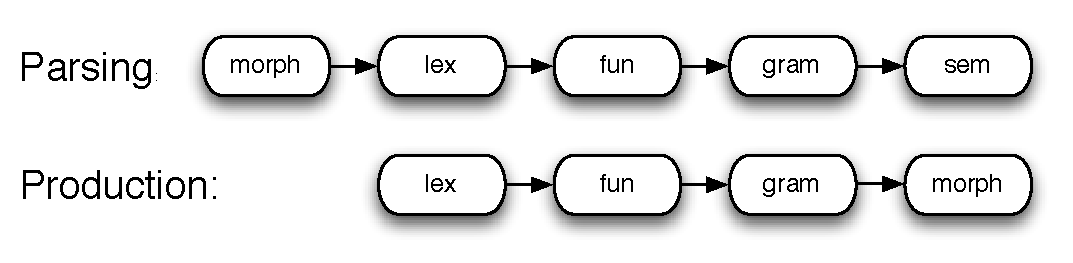
\includegraphics[width=.8\textwidth]{figs/cxn-application}
\end{center}
\caption[Construction application]{%
Construction application in the German spatial language 
grammar discussed in this chapter. In parsing,
morphological constructions apply first followed by lexical and 
grammatical constructions. Finally, the semantic constructions
important for handling semantic ambiguity apply. In 
production, these constructions are 
not applied. In contrast to parsing, morphological constructions apply in 
production at the very end in order to decide on the actual 
form used in the utterance.}
\label{f:construction-application}
\end{figure}

Figure \ref{f:construction-application} shows the sequence of 
construction application in production and in parsing. 
In processing the constructions are part of a 
large pool of constructions, which are applied based on which 
construction can apply at a specific point in time.
Syntactic processing proceeds bottom-up which means from the lexical 
items to the phrasal level. For instance, phrasal constructions require functional 
units to function which in turn depend on lexical constructions. In every
step information is assembled in hierarchical units, e.g. lexical units,
which expose new information, in order, for constructions to use this information.
This process can also be understood as a process of gradual categorization
and assembly of constituents into larger structure both on 
the syntactic and on the semantic side. For instance, lexical constructions
abstract from the concrete semantic entity such as the spatial category 
{\footnotesize\tt left} and provide information about
the semantic type so that functional constructions can use this information
and apply to groups of spatial relations.

The following three sections look in more detail at the implementation
of different constructions such as lexical and functional 
(Section \ref{s:lexical-functional}) phrasal constructions for landmarks
and landmark complements (Section \ref{s:landmarks+complements})
and high-level phrasal constructions (Section \ref{s:phrasal}).
The chapter concludes by discussing how to deal with the German
case system (Section \ref{s:handling-case}).


\section{Lexical classes -- lexical and functional constructions}
\label{s:lexical-functional}
In German the same spatial relation can be expressed using different lexical classes
(adjective, adverb or preposition). The following shows 
an example of the spatial relation {\footnotesize\tt front} expressed
as adjective (Example \ref{e:der-vordere-block-2}), adverb (Example \ref{e:der-block-vorne-2}), 
and prepositions (Example \ref{e:der-block-vor-der-kiste-2}) which
are repeated here for convenience from Chapter \ref{s:german-spatial-language-introduction}.
\ea
\label{e:der-vordere-block-2}
\gll der vordere Block\\
the.{\NOM} front.{\ADJ}.{\NOM} block.{\NOM}\\
\glt `The front block'\\

\z
\ea
\label{e:der-block-vorne-2}
\gll der Block vorne\\
the block.{\NOM} in the front.{\ADV} \\
\glt `The front block'\\

\z
\ea
\label{e:der-block-vor-der-kiste-2}
\gll der Block vor der Kiste \\
the.{\NOM} block.{\NOM} front.{\PREP} the.{\DAT} box.{\DAT} \\
\glt `The block in front of the box'\\

\z

Lexical classes are an example of a many-to-many mappings. 
Every German spatial relation discussed in this book
can be expressed in different lexical classes.
Vice versa, every lexical class has a number of relations that 
are part of it. For instance, the spatial relations {\footnotesize\tt front}, {\footnotesize\tt back}, 
{\footnotesize\tt left}, can all be expressed as adverb. 
However, not all spatial relations can
be expressed as adverbs. The proximal relations \textit{nah} (`near') and \textit{fern} 
do not occur in adverbial form.\footnote{Linguistic analysis is made 
difficult by diverging vocabulary in linguistics and different usages of 
the same term by different schools. I use the term adverb here for spatial relations
such as \textit{vorne} (`front') that can be followed by prepositional phrases and
used as postmodifiers on determined noun phrases e.g. 
\textit{der Block vorne in der Kiste} (`in the front area of the box').}
\tabref{t:lexical-class-word-forms} gives an overview of lexical
classes and associated forms. The table shows that different
groups of spatial relations partake in different lexical classes. 
For instance, all spatial relations except for proximal relations 
such as {\footnotesize\tt near} and {\footnotesize\tt far} can be expressed as
adjectives. Projective relations such as {\footnotesize\tt up}, {\footnotesize\tt front}
and {\footnotesize\tt left} can be expressed as adverbs. Only
vertical and lateral relations can also be genitive prepositions, whereas
frontal relations can only be dative prepositions. Vertical relations can be both 
genitive and dative prepositions. 

\begin{center}
\begin{table}
\begin{centering}
\label{t:lexical-class-word-forms}
\caption[Lexical Classes and word forms for German spatial relations]
{Lexical Classes and word forms for German spatial relations 
(adapted in part from \citealp{tenbrink2007space}\index{Tenbrink, T.}). This by no means
is an exhaustive list of spatial relations, lexical classes or lexical forms 
in German spatial language, but it is the part of German relevant for 
this book. Items marked with * seem to be possible, but due to being
unconfirmed in the reviewed literature are omitted.\newline}
\begin{tabular}{|  p{1.4cm} ||  p{2.0cm} | p{2.0cm}  | p{2.0cm} | p{2.0cm}  | }
\hline
Relation & Adjective & Adverb & Preposition [POSS] & Preposition [DAT] \\\hline\hline
{\footnotesize\tt up} & ober & oben & oberhalb & {\"u}ber \\\hline
{\footnotesize\tt down} & unter & unten & unterhalb & unter\\\hline
{\footnotesize\tt front} & vorder & vorne & & vor \\\hline
{\footnotesize\tt back}  & hinter & hinten  & & hinter\\\hline
{\footnotesize\tt right} & recht & rechts  & rechts & \\\hline
{\footnotesize\tt left} & link & links & links & \\\hline
% {\footnotesize\tt very-near} & &  & & an\\\hline
{\footnotesize\tt near} & * & &  & nahe \\\hline
{\footnotesize\tt far} & * &  & & fern \\\hline
{\footnotesize\tt north}  & n\"ordlich & * & * & n\"ordlich \\\hline
{\footnotesize\tt south} & s\"udlich & * & * & s\"udlich \\\hline
{\footnotesize\tt west} & westlich & * & * & westlich \\\hline
{\footnotesize\tt east} & \"ostlich & * & * & \"ostlich \\\hline
\end{tabular}
\end{centering}
\end{table}
\end{center}

The problem of choosing a lexical class in production and 
finding the lexical class in interpretation is solved by a careful
setup of the interaction of functional and lexical constructions.
I use a particular design pattern called \emph{actual-potential}\index{design pattern!actual-potential}
\footnote{The pattern is inspired by earlier work on
\emph{argument realization} \citep{vantrijp2008phd}\index{van Trijp, R.} which is 
also a many-to-many mapping problem}.
The design pattern allows to store possible lexical classes
in the form of potentials for each lexical item directly in the 
lexical units of the transient structure\index{transient structure}. Subsequent 
functional constructions can constrain their application based on the 
potential of the lexical item, consequently, ruling out 
non standard usage, e.g., expressing proximal relations as adjectives.
The same is used on the semantic side, where the semantic
type hierarchy of the semantic entity is stored as a list of potentials.

The \emph{actual-potential}\index{design pattern!actual-potential} technique allows to 
distribute decision making across lexical and functional constructions 
by separating the specification of options (\emph{potentials})
from the \emph{actual} decision. Possible choices are
explicitly stored in the form of disjunctive potentials
in the transient structure 
thereby signaling to subsequent constructions which choices are 
possible which allows subsequent constructions to constrain their 
application by observing potentials and triggering only when
the right potentials are present. Before we jump to the 
application of the actual-potential\index{design pattern!actual-potential} design pattern, we need to 
consider the lexical and functional constructions that are involved.

The fact that Examples \ref{e:der-vordere-block-2}, 
\ref{e:der-block-vorne-2} and \ref{e:der-block-vor-der-kiste-2} 
refer to the same projective category {\footnotesize\tt front} is expressed 
by the lexical construction for the spatial relation {\footnotesize\tt front}.
The construction maps the reference to the spatial relation onto 
the word stem \textit{vor}. The following template shows the lexical 
construction for the category {\footnotesize\tt front}:
\ea
\label{e:def-lex-front}
\begin{footnotesize}
\begin{Verbatim}[commandchars=\\\{\}]
(def-lex-cxn
 (def-lex-skeleton front-cxn 
  :meaning (== (bind frontal-category ?cat front)) 
  :args ((ref ?cat))
  :stem "vor"))
\end{Verbatim}
\end{footnotesize}
\z
Lexical constructions capture the similarity of different syntactic and
semantic usage scenarios of the same category. They encode
that no matter how the lexical item is used in the larger
semantic and syntactic structure it refers to the same
semantic entity, e.g., spatial relation.

Functional constructions map a particular lexical 
class to syntactic and semantic properties thereby
elevating lexical items to constituents in grammatical structure. 
On the semantic side, functional constructions trigger on semantic operations 
used in conceptualization. On the syntactic side, the constructions 
provide syntactic functions and syntactic classes in order for grammatical constructions 
to be able to build grammatical structure out of functional units.
Below are the skeletons for the functional constructions of spatial 
adjective, frontal adverbs and frontal prepositions:

\ea
\label{e:def-fun-spatial-adjective}
\begin{footnotesize}
\begin{Verbatim}[commandchars=\\\{\}]
(def-fun-cxn spatial-adjective 
 :meaning (== (apply-spatial-category-group-based 
                ?target ?source ?category))
 :args ((ref ?target)(src ?source)(cat ?category))
 :sem-function (modifier)
 :syn-function (adjectival))
\end{Verbatim}
\end{footnotesize}
\z

\ea
\label{e:def-fun-frontal-adverb}
\begin{footnotesize}
\begin{Verbatim}[commandchars=\\\{\}]
(def-fun-cxn frontal-adverb 
 (def-fun-skeleton frontal-adverb
  :meaning (== (construct-region-frontal-internal
           ?target ?source ?landmark ?category ?f-o-r))
  :args ((ref ?target)(src ?source)
           (cat ?category)(landmark ?landmark))
  :sem-function (modifier)
  :sem-class (region internal-region relative-region)
  :syn-function (adverbial)
  :syn-class (adverb)))
\end{Verbatim}
\end{footnotesize}
\z

\ea
\label{e:def-fun-frontal-preposition}
\begin{footnotesize}
\begin{Verbatim}[commandchars=\\\{\}]
(def-fun-cxn frontal-preposition
 (def-fun-skeleton frontal-preposition
  :meaning (== (construct-region-frontal 
             ?target ?source ?landmark ?category ?f-o-r))
  :args ((ref ?target)(src ?source)
           (cat ?category)(landmark ?landmark))
  :sem-class (angular-relationship)
  :syn-class (angular-preposition)))
\end{Verbatim}
\end{footnotesize}
\z

These constructions introduce constructional meaning, e.g. 
{\footnotesize\tt construct-region-frontal} together with semantic 
and syntactic potentials. One is the functional role of the
unit in the larger syntactic structure, here denoted by 
{\footnotesize\tt syn-function}. Aside from these two constructions, there are 
a number of other important functional constructions. 
In particular the difference in semantics of
lateral and frontal adverbs, but also between projective, topological
and absolute relations are each captured by separate 
functional constructions (see Table \ref{t:functional-constructions} for an overview).

\begin{sidewaystable}
%\begin{table}
\begin{footnotesize}
\begin{tabular}{| p{1.5cm} || p{1.1cm} | p{1.45cm} || p{1.7cm} || p{1.9cm} | p{1.55cm} | p{1.45cm} | p{1.5cm} || p{1.9cm} |}
\hline
name & lex-type & lex-cat & operation & sem-functions & sem-classes & syn-functions & syn-classes & examples 
% \\ \hline \hline
% color-adjective-cat  &color &color-adjective & apply-color-category &modifier & &adjectival & &gr\"un, rot 
\\ \hline \hline 
spatial-adjective-cat  &spatial-category &spatial-adjective & apply-spatial-category-group-base &modifier & &adjectival & &linke, rechte, vordere, hintere
\\ \hline
frontal-adverb  &frontal-category &frontal-adverb  & construct-region-frontal &modifier &relative-region, frontal-region, region &adverbial &frontal-adverb, adverb &vorne, hinten 
\\ \hline 
frontal-preposition  &frontal-category & frontal-preposition & construct-region-internal & & angular-relationship & & angular-preposition &vor, hinter 
\\ \hline 
spatial-preposition-cat  &spatial-category &spatial-preposition & construct-region-proximal &relationship & &preposition & &an 
\\ \hline 
lateral-adverb--preposition  &lateral-category &lateral-adverb--preposition & construct-region-lateral &modifier &relative-region, angular-relationship, ... &adverbial &lateral-adverb, angular-preposition, ... &links, rechts 
\\ \hline 
noun-cat  &object-class &noun & apply-object-class &identifier & &nominal & &block, kiste 
% \\ \hline 
%pronoun-cat  &discourse-role & pronoun & identify-discourse-participant &reference & &referring-expression & &mir, dir 
\\ \hline 
article-cat  &selector &article & apply-selector &determiner & &determiner & &der,die,das 
\\ \hline
\end{tabular}
\caption[Functional constructions]
{Overview of a subset of the functional constructions of the German grammar. 
The three columns {\footnotesize\tt lex-type},
{\footnotesize\tt lex-cat} and {\footnotesize\tt operation} show the requirements for each construction.
The four columns {\footnotesize\tt sem-functions}, {\footnotesize\tt sem-class}, {\footnotesize\tt syn-functions}
and {\footnotesize\tt syn-classes} detail the syntactic and semantic functions and classes that
the constructions introduce.}
\label{t:functional-constructions}
%\end{table}
\end{footnotesize}
\end{sidewaystable}

\begin{figure}
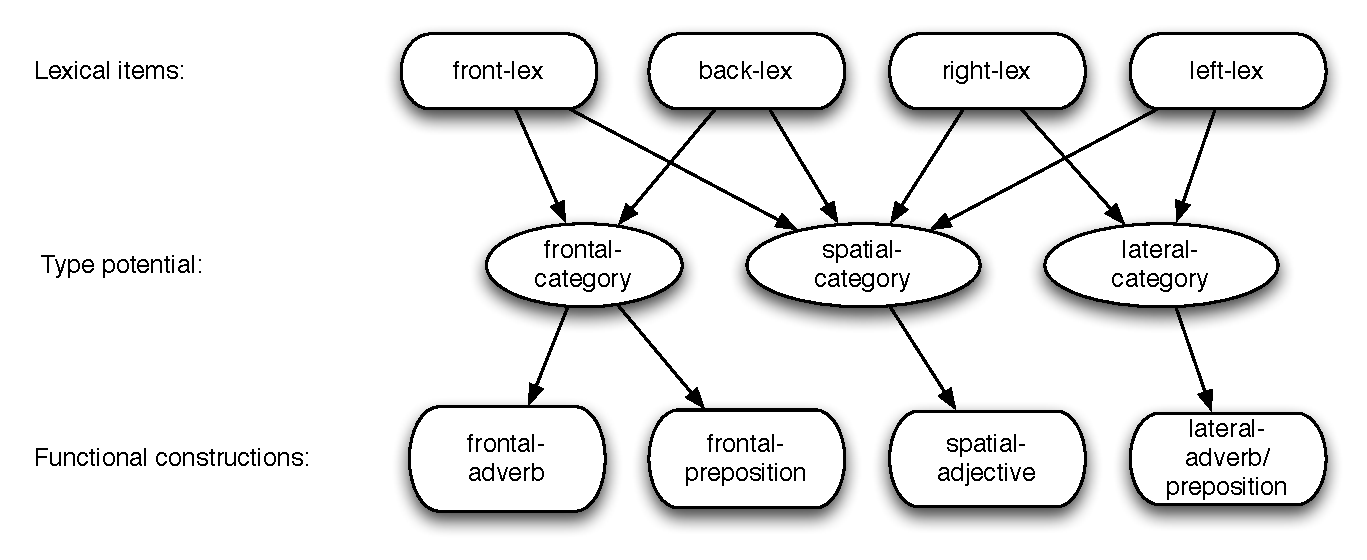
\includegraphics[width=\columnwidth]{figs/lexicals-type-potentials-cats}
\caption{Subset of the mapping of lexical items to functional constructions.}
\label{f:lexicals-type-potentials-cats}
\end{figure}

\subsection{Encoding type and lexical class potentials}
In order to solve the many-to-many mapping problem,
lexical and functional constructions are 
extended using the \emph{actual-potential}\index{design pattern!actual-potential} design pattern 
on the syntactic and semantic pole of constructions.
Lexical constructions merge semantic and 
syntactic potentials into lexical units. This 
information is used by functional constructions 
to constrain their application. On the 
semantic side, the {\footnotesize\tt type} constraints are rooted 
in the type hierarchy of spatial relations, whereas on the
syntactic side, the lexical class {lex-cat} potential encodes
which functional constructions can apply. 
The constraints take the form of disjunctive lists of potentials.
For example, since all angular categories, i.e. projective and absolute
categories, can be used as adjectives, the lexical constructions for these 
categories feature the {\footnotesize\tt type} potential {\footnotesize\tt angular-spatial-category}, 
as well as the syntactic {\footnotesize\tt lex-cat} potential 
{\footnotesize\tt spatial-adjective}. The adjective construction
constrains itself to only apply to lexical units that have this 
potential thereby licensing the application of the spatial adjective
construction. The lexical units for proximal relations, such
as {\footnotesize\tt near} and {\footnotesize\tt far} do not have these potentials, hence,
the adjective construction cannot apply.
Other fine-grained distinctions can be modeled as well.
Lateral and frontal projective categories differ in how their 
corresponding adverbs behave syntactically and semantically
which necessitates two functional constructions, one for lateral adverbs and one 
for frontal adverbs. Consequently, the potentials in frontal category units 
differ from lateral ones. They feature the type {\footnotesize\tt frontal-category}, 
where lateral lexical constructions (i.e. for {\footnotesize\tt left} and {\footnotesize\tt right})
provide the {\footnotesize\tt type} potential {\footnotesize\tt lateral-category}
(see Figure \ref{f:lexicals-type-potentials-cats} 
for {\footnotesize\tt type}  potentials of projective lexical constructions and
Figure \ref{f:lexicals-lex-cat-potentials-cats}  for {\footnotesize\tt lex-cat} potentials)

\begin{figure}
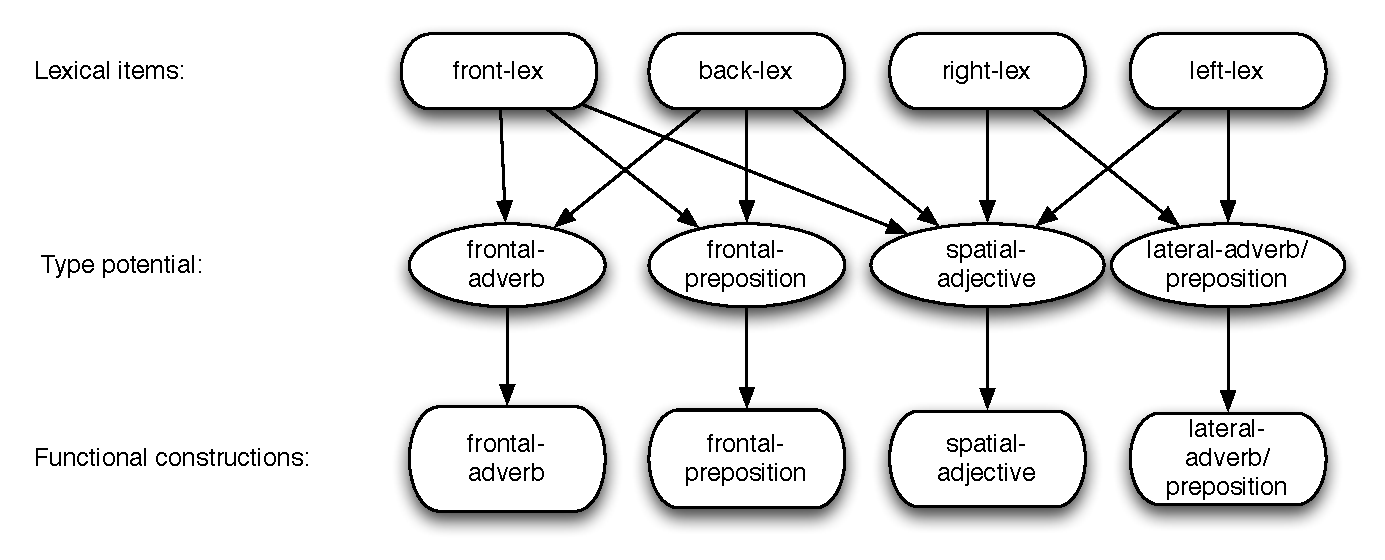
\includegraphics[width=\columnwidth]{figs/lexicals-lex-cat-potentials-cats}
\caption{Subset of the mapping from lexical items to functional constructions.}
\label{f:lexicals-lex-cat-potentials-cats}
\end{figure}

\subsection{Technical realization}
The actual-potential\index{design pattern!actual-potential} design pattern is easily implemented
using a dedicated template for extending lexical constructions.
Example \ref{e:def-lex-front}, for instance, is supplemented by the following two 
templates which introduce potentials on the semantic and syntactic side.
\ea
\label{e:def-lex-front-potentials}
\begin{footnotesize}
\begin{Verbatim}[commandchars=\\\{\},fontsize=\footnotesize]
(def-add-potential front sem sem-cat type 
 (angular-spatial-category 
  projective-category 
  frontal-category))
(def-add-potential front syn syn-cat lex-cat 
 (spatial-adjective frontal-adverb frontal-preposition))
\end{Verbatim}
\end{footnotesize}
\z
These two templates specify the {\footnotesize\tt type} and 
{\footnotesize\tt lex-cat} potentials and directly translate into 
attributes in the {\footnotesize\tt front} lexical construction:
\ea
\label{e:def-lex-front-cxn}
\begin{footnotesize}
\begin{Verbatim}[]
(...
 (J ?front-unit ?top ()
  ...
  (sem-cat 
   (== 
    (type 
     ((actual ?type-value)
      (potential 
       (angular-spatial-category 
        projective-category 
        frontal-category)))))
   ...)
...)
 <-->
(...
 (J ?front-unit ?top ()
  ...
  (syn-cat 
   (== 
    (lex-cat
     ((actual ?lex-cat-value)}
      (potential 
       (spatial-adjective 
        frontal-adverb 
        frontal-preposition))))
    ...))
...)
\end{Verbatim}
\end{footnotesize}
\z
Importantly, the template {\footnotesize\tt def-add-potential} 
not only adds the {\footnotesize\tt potential} attribute but also an 
attribute called {\footnotesize\tt actual}. This attribute, as we will
see in the next paragraphs, is automatically set to a variable 
in the lexical construction and is used to store which 
{\footnotesize\tt type} attribute is used. If one of the potentials 
is picked up, for instance by a functional construction, the 
{\footnotesize\tt actual} attribute is also set.

The information stored by the lexical construction in the transient structure\index{transient structure}
allows functional constructions to choose 
the potential in which they are interested and to constrain
their own application. This process can be seen in an extended 
version of the functional spatial adjective construction:
\ea
\label{e:def-fun-spatial-adjective-potentials}
\begin{footnotesize}
\begin{Verbatim}[commandchars=\\\{\}]
(def-require-potential spatial-adjective 
  ?cat-unit sem sem-cat 
 type angular-spatial-category)
(def-require-potential spatial-adjective 
 ?cat-unit syn syn-cat
 lex-cat spatial-adjective)
\end{Verbatim}
\end{footnotesize}
\z
These templates express that, in order for the spatial adjective 
construction to apply, certain potentials need to be present in the 
transient structure\index{transient structure}. More precisely, the {\footnotesize\tt type} potential 
{\footnotesize\tt angular-spatial-category} and the {\footnotesize\tt lex-cat} potential 
{\footnotesize\tt spatial-adjective} need to be there. 

The template for spatial adjectives translates into the following 
feature structure (for illustrative purposes, only the semantic 
side is shown here):
\ea
\label{e:def-fun-spatial-adjective-potentials}
\begin{footnotesize}
\begin{Verbatim}[commandchars=\\\{\}]
(...
 (?cat-unit
  (sem-cat 
   (== 
    (type
     ((actual angular-spatial-category)
      (potential 
       (==! angular-spatial-category))))
    ...))
...)
\end{Verbatim}
\end{footnotesize}
\z
This construction can only apply if the {\footnotesize\tt type} potential 
of the lexical constituent in the transient structure imperatively includes 
{\footnotesize\tt angular-spatial-category}. Additionally,
it requires the {\footnotesize\tt actual} attribute
to be {\footnotesize\tt angular-spatial-category} or a variable. There are two
things to note here: the use of the {\footnotesize\tt ==!} operator for 
potentials and the handling of the {\footnotesize\tt actual} attribute. 
The {\footnotesize\tt ==!} operator only unifies and never merges, 
which means that neither in production nor parsing can a missing 
potential be merged. The specified potential always has to be present, 
in this case on the semantic side, but for the {\footnotesize\tt lex-cat} 
potentials, the case is vice versa on the 
syntactic side. Consequently, choosing a potential does not 
change the potential in the transient structure\index{transient structure}. 
The second feature, the {\footnotesize\tt actual} attribute must be equal 
to {\footnotesize\tt angular-spatial-category} or a variable, in order for the spatial 
adjective construction to apply. If the attribute
is a variable, then that variable is bound to {\footnotesize\tt angular-spatial-category}, 
and, hence, the application of the spatial adjective construction 
modifies the transient structure and sets the {\footnotesize\tt value} attribute 
to the required potential. Of course, the corresponding potential also 
has to be present for the construction to
apply in the first place (see Figure \ref{f:production-vordere})

\begin{figure}
\begin{center}
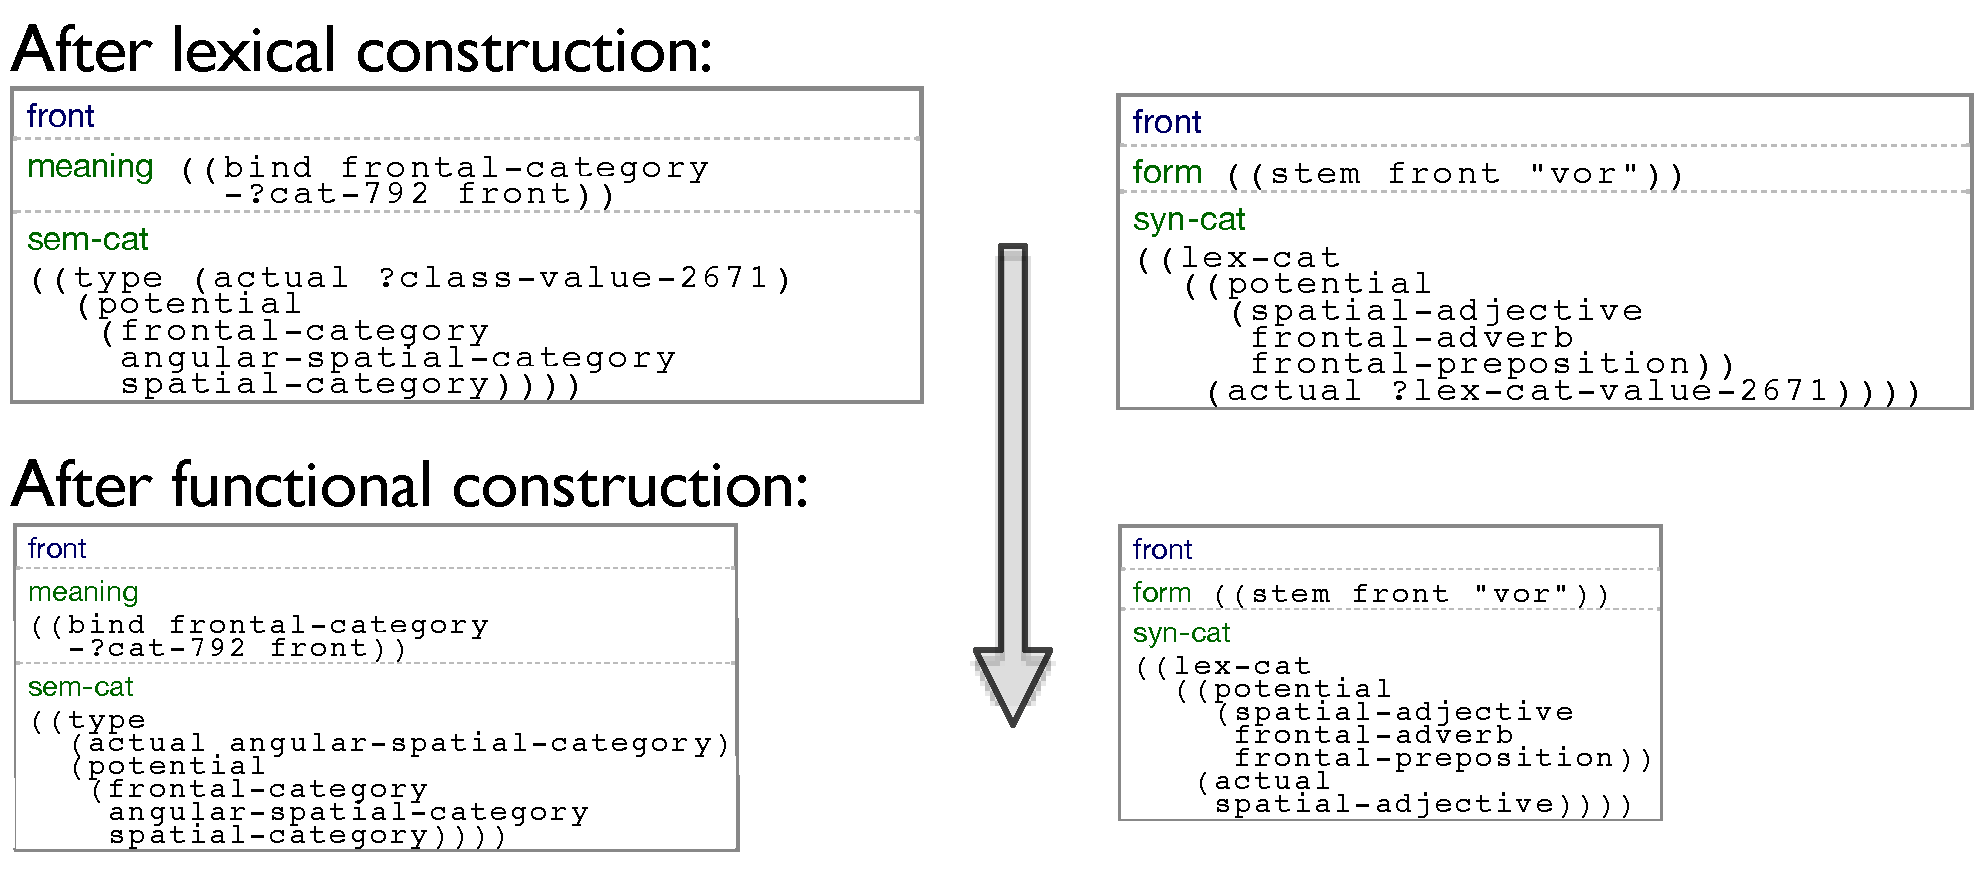
\includegraphics[width=1.0\columnwidth]{figs/production-vordere}
\end{center}
\caption[Interaction of lexical and functional constructions -- syntax]{
Interaction of lexical constructions with 
functional constructions in production of
\textit{vordere} (`front').
The arrow signifies the order of application. 
Left, the {\footnotesize\tt vordere} unit on the semantic side of the 
processed transient structure is shown. 
Right, the syntactic unit is shown. The 
transient structure\index{transient structure} actually contains more units, and the units 
themselves contain more features, but
everything has been shortened for illustrative purposes. The 
top row shows the lexical unit after
the application of lexical constructions, which have equipped 
the lexical unit with potentials
for {\footnotesize\tt type} on the semantic side, and {\footnotesize\tt lex-cat}  
on the syntactic side. Both of
these potentials have no value assigned to them yet. It is only 
after the application of the functional
construction of spatial adjective that both have values assigned 
to them, {\footnotesize\tt spatial-category}
for {\footnotesize\tt type} and {\footnotesize\tt spatial-adjective} for {\footnotesize\tt lex-cat}.}
\label{f:production-vordere}
\end{figure}

\begin{figure}
\begin{center}
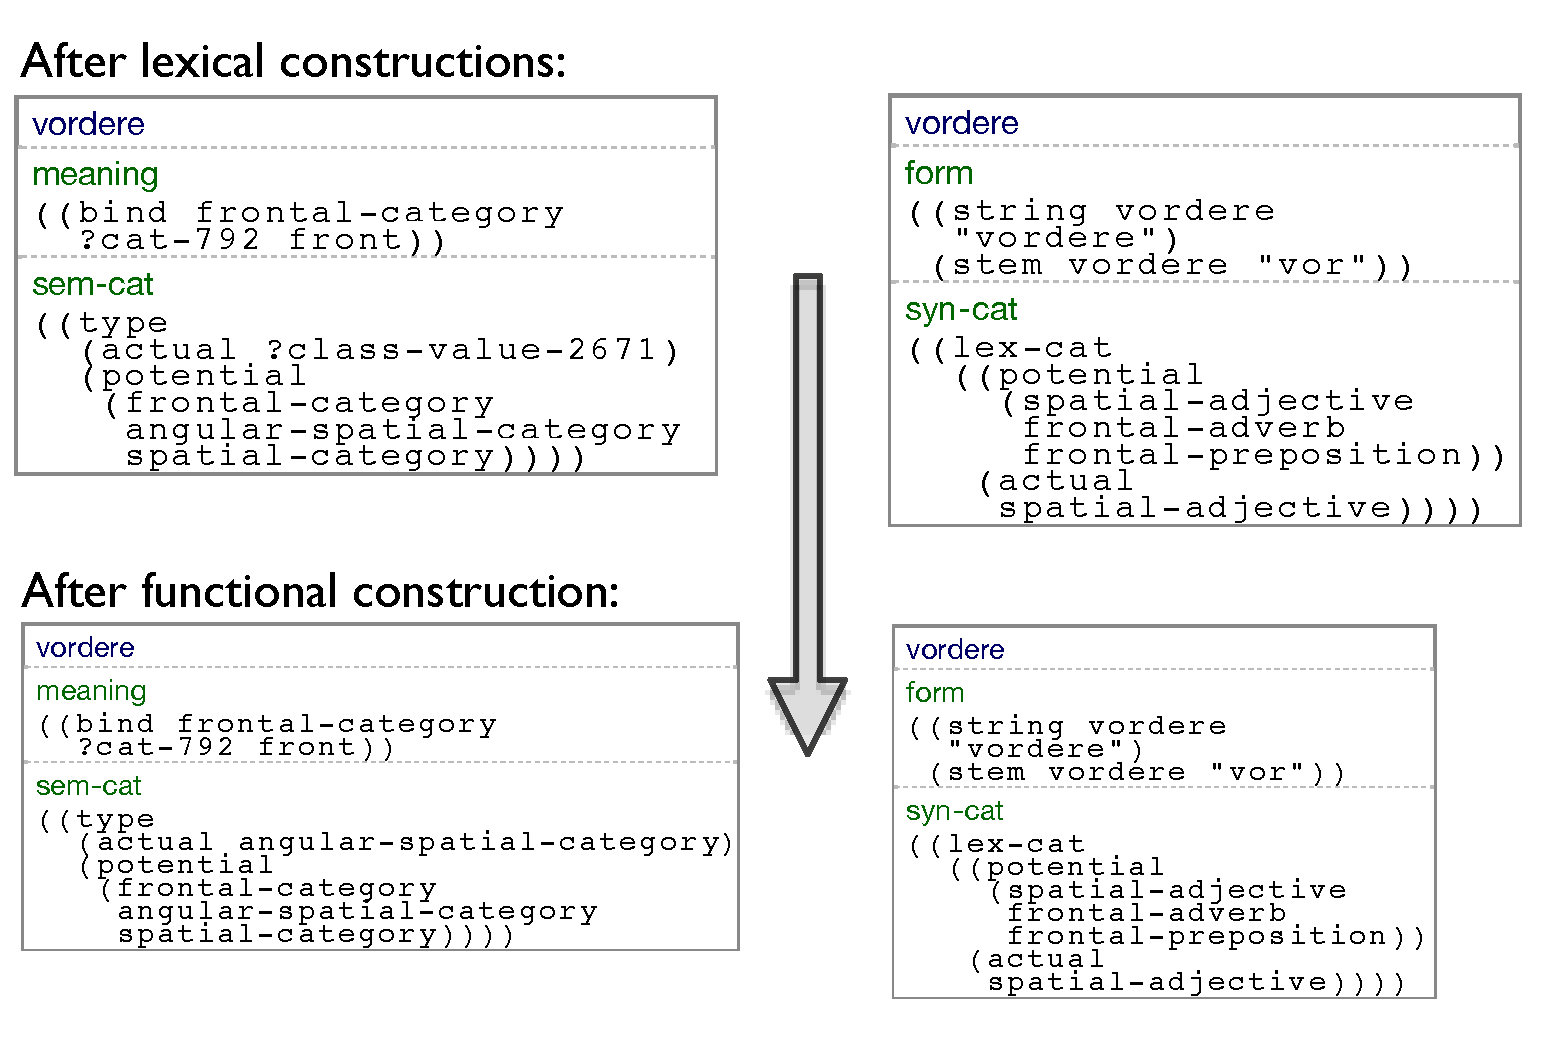
\includegraphics[width=1.0\columnwidth]{figs/parsing-vordere}
\end{center}
\caption[Interaction of lexical constructions
with functional constructions -- semantics]{
Interaction of lexical constructions 
with functional constructions in parsing \textit{vordere} (`front'). 
Lexical constructions apply before functional constructions.
The {\footnotesize\tt vordere} unit on the semantic side of the 
processed transient structure\index{transient structure} is shown on the left.
The syntactic unit is shown on the right. The transient 
structure actually contains more units, and the units themselves
contain more features, but everything has been shortened 
for illustrative purposes. The top row shows the lexical unit after the 
application of morphological and lexical constructions. The 
parsed string unambiguously allows for a decision to be 
made on the {\footnotesize\tt lex-cat} value, and 
hence the value is set on the syntactic side. It is the functional 
construction that picks one of the {\footnotesize\tt potential} {\footnotesize\tt types} 
on the semantic side and 
fills its {\footnotesize\tt value} attribute.}
\label{f:parsing-vordere}
\end{figure}

% explain interaction with morph rules 
This split into {\footnotesize\tt value} and {\footnotesize\tt potential} and 
the ability to interact via these two attributes is not only interesting
for grammar designers who can track the application
of constructions by tracing the actually chosen potential, but, it plays 
an active role in processing. In parsing,
the lexical class of a word is decided by morphological 
constructions. The morphological constructions apply first when 
parsing an utterance and they provide a value for the
{\footnotesize\tt actual} attribute. For instance, when observing the form 
\textit{vorne}, the morphological construction responsible for the
string \textit{vorne} triggers and adds the information to the transient 
structure, namely that an adverb was observed in parsing (see 
\figref{f:parsing-vordere} for a schematic overview).

\subsection{Discussion}
Handling the many-to-many mapping problem in lexical class choice
in principle also has other solutions. In particular, one could
rely on the search process of FCG in order to branch into all possible
lexical classes for a particular lexical item, and cut branches until only the 
one relevant for the current purpose, e.g. for the meaning produced, survives. 
This solution requires one lexical constructions for each possible lexical class
and for each category. This leads to excessive branching in search. 
The solution presented in this chapter does not require branching
in search and is thus more efficient. Another solution to this problem,
is to code the interaction of lexical items and lexical classes in a holistic
fashion which means that every possible combination of lexical class 
and lexical item is represented by exactly one construction. This 
solution does depend on branching of search, but demands grammar
designers to hand code many constructions (for the case discussed in
this chapter more than 30 combined constructions are needed). 
The solution presented in this chapter leads to a concise grammar,
with much fewer constructions (less than 20 lexical and functional constructions).


%%%%%%%%%%%%%%%%%%%%%%%%%%%%%%%%%%%%
\section{Landmarks and complements -- 
adverbial and prepositional constructions}
\label{s:landmarks+complements}
Chapter \ref{s:german-spatial-language-introduction} contains a number of 
examples of landmark and perspective marking in German spatial 
phrases. Most importantly I concluded that in spatial prepositional phrases 
the landmark is always part of the prepositional phrase. This contrasts 
with adverbs which allow landmarks to be expressed optionally
using prepositional complements. Additionally, we have seen in Chapter 
\ref{s:german-space-semantics} how spatial semantics chiefly relies on particular 
semantic operations and linking of semantic structure. Consequently, 
there are two important questions related to processing landmarks and 
perspective in adverbial and prepositional phrases: 1) how to deal with 
optional elements in a concise way, and 2) how to achieve linking. 
In this section I explore the solution to these problems for projective categories, 
in particular projective adverbs and projective prepositions. 


\begin{sidewaystable}
\begin{centering}
\begin{footnotesize}
\begin{tabular}{| p{1.6cm} || p{1.6cm} | p{1.6cm}  || p{1.6cm} | p{1.6cm}  || p{1.4cm} | p{1.4cm}  || p{3.5cm} |}
\hline
cxn &  c1 syn-function & c1 syn-class &  c2 syn-fn & c2 syn-class  & syn-functions & syn-classes & examples \\ \hline\hline
angular-pp-phrase & & angular-preposition & referring-expression & & adverbial & &[vor] [der Kiste], [links] [der Kiste]
\\ \hline  
lateral-region-landmark-marked  & adverbial &adverb & referring-expression & & adverbial & & [links] [von mir] 
\\ \hline  
relative-region-perspective-marked  &adverbial & &referring-expression & & & &
[vor der kiste] [von mir aus], [links] [von mir aus], [links von der Kiste] [von mir aus] 
\\ 
\hline
\hline
cxn name &  c1 sem-function & c1 sem-class &  c2 sem-fn & c2 sem-class  & sem-functions & sem-classes & examples \\ \hline\hline
angular-pp-phrase & & angular-relationship & reference & & modifier & region, relative-region & [vor][der Kiste], [links][der Kiste]
\\ \hline
lateral-region-landmark-marked  & modifier & lateral-region & reference & & modifier & region, relative-region & [links] [von mir] 
\\ \hline
relative-region-perspective-marked  & modifier & relative-region &reference & &modifier & region &
[vor der Kiste] [von mir aus],[links] [von mir aus], [links von der Kiste] [von mir aus] 
\\ \hline
\end{tabular}
\end{footnotesize}
\end{centering}
\label{t:landmark-perspective-cxns}
\caption[Syntactic and semantic mappings of constructions]{
Syntactic and semantic mappings of constructions 
governing prepositional and complemented adverbials. Syntactic and semantic
functions and classes for the two constituents (c1 and c2) are shown. To the right
the newly introduced syntactic and semantic function and classes are shown.}
\end{sidewaystable}

Let us first consider the extension of projective prepositions 
using a landmark. The construction handling projective and absolute 
prepositions is called {\footnotesize\tt angular-pp-phrase}. It has two constituents
(see Table \ref{t:landmark-perspective-cxns}) . 
The first constituent is one that has the semantic 
class {\footnotesize\tt angular-relationship} and the syntactic class 
{\footnotesize\tt angular-preposition} (see Table 
\ref{t:functional-constructions} and in particular the semantic and 
syntactic function attributes of all projective 
prepositional constructions {\footnotesize\tt frontal-preposition},
{\footnotesize\tt lateral-preposition} and {\footnotesize\tt vertical-preposition})
functional construction). The second constituent is 
the landmark. For the landmark there are only functional constraints. 
Whatever is supposed to act as the landmark needs to be some kind of
{\footnotesize\tt reference} (semantic) and {\footnotesize\tt referring-expression} (syntactic). 
How is the linking precisely achieved? 
When we look at the prepositional construction in Example 
\ref{e:def-fun-frontal-preposition}, we see that it features the variable 
{\footnotesize\tt ?landmark} connected to the landmark slot of the respective 
operation. Since FCG cannot rely on variable names as they 
might change, the variable is repeated in the {\footnotesize\tt args} feature, 
clearly marked in the attribute {\footnotesize\tt landmark}. 
This means, that the {\footnotesize\tt angular-pp-phrase} construction, 
can unify with this specific argument, which is  for this purpose. 
Let us look at the template to understand the linking

\ea
\begin{footnotesize}
\begin{verbatim}
(def-phrasal-cxn angular-pp-phrase
 :constituents
 (def-constituent
  :syn-class angular-preposition 
  :sem-class angular-relationship
  :args ((landmark ?landmark)))
 (def-constituent
  :syn-function referring-expression
  :sem-function reference
  :args ((ref ?landmark)))
  :syn-function adverbial
  :sem-function modifier)
\end{verbatim}
\end{footnotesize}
\label{e:angular-pp-phrase}
\z
Linking is achieved by explicitly unifying the corresponding 
{\footnotesize\tt args} in the structure, using the variable
{\footnotesize\tt ?landmark}. The variable occurs both in the {\footnotesize\tt ?ref} 
argument of the {\footnotesize\tt reference} constituent 
and the {\footnotesize\tt landmark} argument of the 
{\footnotesize\tt angular-relationship} constituents. 


For adverbs the linking with landmark works similar to prepositions. 
However, there are important differences in syntax between prepositions
and adverbs. Let us consider the example of lateral adverbs.
Lateral adverbs can be extended by landmarks, but the has to 
be marked using a \textit{von} prepositional phrase. 
The construction handling the landmark augmentation of lateral adverbs 
is shown below. In addition to linking, this construction introduces
the preposition \textit{von}. 


\ea
\begin{footnotesize}
\begin{verbatim}
(def-phrasal-cxn lateral-adverb-landmark-marked
 :constituents
 (def-constituent
  :syn-function adverbial
  :syn-class lateral-adverb 
  :sem-function modifier
  :sem-class lateral-region
  :args ((landmark ?landmark)))
 (def-constituent
  :syn-function referring-expression
  :sem-function reference
  :args ((ref ?landmark))
  :preposition "von")
 :syn-function adverbial
 :sem-function modifier)
\end{verbatim}
\end{footnotesize}
\label{e:lateral-adverb-landmark-marked}
\z


These two constructions show how to solve parts of the  
complexity puzzle of the interaction of syntax and semantics, 
i.e. the linking issue, while at the same time they deal with the syntactic 
differences for adverbs (in this case only lateral adverbs are discussed, 
but similar constructions exist for vertical and frontal adverbs) and 
prepositions. Moreover, the two constructions also 
prevent frontal adverbs from being 
landmark augmented by any of the two constructions, 
since frontal adverbs do not have
the {\footnotesize\tt angular-preposition} potential, but also they 
cannot be extended using the lateral 
landmark marking scheme, since they are not of class 
{\footnotesize\tt lateral-region}. Other constructions deal with 
\textit{in} prepositional phrases and frontal adverbs.

\begin{table}
\begin{centering}
\begin{tabular}{| p{2.0cm} || p{1.8cm} || p{1.8cm}  || p{1.8cm}  || p{2.3cm} |}
\hline
cxn &  c1 syn-fn & c2 syn-fn & syn-fns & examples \\ \hline\hline
adjectival--nominal--phrase  &adjectival & nominal & nominal & [linke] [block] 
 \\ \hline  
determiner--nominal--phrase  &determiner & nominal & referring-expression & [der] [block] 
\\ \hline 
referring-expression-adverbial-phrase  &referring-expression & adverbial & referring-expression & [der block] [links], [der block] [vor/an...] 
\\ \hline  
preposition--referring-expression--phrase  &preposition & referring-expression & adverbial & [an][der kiste] 
\\ \hline  
possessive  &referring-expression & referring-expression & referring-expression & [die linke Seite] [der Kiste] 
\\ \hline
\end{tabular}
\caption[Mapping of syntactic functions]{Mapping of syntactic functions (phrasal constructions). All phrasal
constructions have two constituents and all build hierarchical structure by subsuming the two constituents (\emph{c1} and 
\emph{c2}) into a new unit. 
Columns \emph{c1 syn-fns} and \emph{c2 syn-fns} show the syntactic function potential expected from constituents.
The column \emph{syn-fns} details the syntactic function potential of the new unit. All constructions shown here
introduce word order and require the first constituent \emph{c1} to meet the second
constituent \emph{c2}, i.e. \emph{c1} has to be exactly before \emph{c2}.}
\label{t:phrasal-syn}
\end{centering}
\end{table}

\section{Linking everything together -- high-level phrasal constructions}
\label{s:phrasal}
The previous section looked at prepositional and adverbial constructions. 
But, there is more. Particularly, there are important constructions, which only care 
about the syntactic and semantic functions of their constituents, and hence are 
widely applicable and underly the ability of the grammar to build and parse 
complex recursive utterances involving many complemented phrases. Phrasal 
constructions have two constituents. The unification of constituents is based on 
the actual-potential\index{design pattern!actual-potential} design pattern. The constructions require their constituents 
to provide certain semantic and syntactic function potentials, while providing 
new potentials for semantic and syntactic functions themselves. 
All of them also introduce a particular word order and a particular linking 
of the arguments of their constituents and the meaning they express. They internally link
the arguments of constituents while providing new arguments themselves.
Hence, in production these constructions express particular linkings in the semantic structure using a particular word order. Vice versa, in parsing they introduce links in the semantic structure when observing a particular word order
of their functional constituents. 

The simplest example of such a construction is the {\footnotesize\tt adjectival-nominal-phrase}, which allows agents to build large adjective noun phrases 
(see \citealp{steels2011phrasal}\index{Steels, L.} for the original idea). 
Tables \ref{t:phrasal-syn} 
and \ref{t:phrasal-sem} detail the semantic and syntactic functions of 
the constituents of all phrasal constructions, as well as the syntactic 
and semantic function potentials they introduce. The adjectival 
nominal construction maps a constituent with syntactic 
function {\footnotesize\tt adjectival} and semantic function {\footnotesize\tt modifier} and a constituent with syntactic function nominal and semantic function identifier onto a new unit. Hence, it builds hierarchy by introducing a new unit with two subunits 
namely its two constituents. This new unit has the semantic function potential of identifier and the syntactic function 
potential nominal. There are a number of functional constructions providing such semantic and syntactic 
functions. Both color and spatial adjectives provide the semantic function {\footnotesize\tt modifier} and the syntactic
function {\footnotesize\tt adjectival}. The semantic function {\footnotesize\tt identifier} and the syntactic function {\footnotesize\tt nominal} are provided by nouns. Hence, when encountering such constituents in production, for instance, because noun and adjective functional constructions have provided suitable constituents, the construction will form a new unit with semantic function 
nominal and introduce the German word order, where adjectives always come before the 
noun. This new structure can itself be considered functionally equal to nouns, as it features the same syntactic and 
semantic functions. It therefore can be subject to modification through other adjectives. Finally, units that have the
semantic function {\footnotesize\tt identifier} and the syntactic function {\footnotesize\tt nominal},
can be extended by determiners through application of the {\footnotesize\tt determiner-nominal-phrase}, which results in a unit that encapsulates the semantic function 
{\footnotesize\tt reference} and the syntactic function {\footnotesize\tt referring-expression} and
provides for all examples, where nouns, or adjective modified nouns are determined
using an article.
\begin{table}
\begin{tabularx}{\textwidth}{XXXXXX}
\lsptoprule
cxn &  c1 sem-fn & c2 sem-fn & sem-fns & operation  & examples\\
\midrule
adjectival--nominal--phrase  &modifier &identifier &identifier & &[linke] [block] 
\\ \midrule
determiner--nominal--phrase  &determiner & identifier & reference & & [der] [block] 
\\ \midrule
preposition--referring-expression--phrase &relation &reference & modifier &  & [an] [der kiste] 
\\ \midrule 
referring-expression-adverbial-phrase  & reference & modifier & reference & 
apply-region-filter & [der block] [links], [der block] [vor/an...] 
\\ \midrule 
possessive  & reference & reference & ref & possessive
& [die linke Seite] [der Kiste] 
\\\lspbottomrule
\end{tabularx}
\caption[Mapping of semantic functions]{Mapping of semantic functions of phrasal constructions. For every construction the semantic function 
potential that needs to be present for the two constituents \emph{c1} and \emph{c2} is shown, as well as the 
new semantic function potential provided (\emph{sem-fns}). Some of the constructions add additional meaning
with more complicated argument linking properties. All others however link the {\footnotesize\tt ref} argument of constituent two (\emph{c2}) to the {\footnotesize\tt source} argument of constituent one (\emph{c1}).}
\label{t:phrasal-sem}
\end{table}

This explains how adjectival noun phrases can be build, 
but how do adverbial complement phrases discussed in the 
previous section get linked to referring expressions? 
This is solved by the {\footnotesize\tt referring-expression-adverbial-phrase}, 
which links constituents with semantic/syntactic function 
{\footnotesize\tt reference/referring-expression} (example \textit{der block} or \textit{der gr\"une Block}
and {\footnotesize\tt modifier/adverbial} (example \textit{links}, \textit{links von der Kiste}, 
\textit{vor der Kiste} \ldots) into a unit that not only syntactically introduces 
the word order, that the adverbial is behind the referring expression, 
but also links the meaning and adds the operation {\footnotesize\tt apply-region-filter}. 
This construction besides linking the meaning of constituents, additionally, 
adds an operation that is applied to the output of the meaning 
of the adverbial phrase. Here, this operation is {\footnotesize\tt apply-region-filter}, which 
filters the context given a particular region. It is important to understand, 
that this particular construction can be so general only because 
all complements in the grammar compute regions. In other words all adverbial complements, be they prepositional phrases or adverbials or complemented adverbials always denote a spatial region. 
The {\footnotesize\tt referring-expression-adverbial-phrase} construction, that handles 
all adverbial complements of determined nominal phrases, only needs to care about 
modifiers and, hence, its generality is based on the fact, that semantically 
all adverbial complements in this grammar compute regions, while observing 
a particular word order. If there would be other possible complements, this 
construction would also need to specialize on the semantic type of the constituents.

%%%%%%%%%%%%%%%%%%%%%%%%%%%%%%%%%%%%
%\section{Handling Semantic Ambiguity (on the Level of Grammar) -- Perspective Marking or Not?}
%\label{s:semantic-ambiguity}


%%%%%%%%%%%%%%%%%%%%%%%%%%%%%%%%%%%%
\section{Handling case}
\label{s:handling-case}
Case and gender agreement in German is an example of a 
highly distributed information
processing task. The constraints on these syntactic features 
are contributed by many different constructions 
and thus have to be incrementally integrated in order
to produce grammatical utterances in German. For instance, the
grammatical gender of a prepositional determined adjective noun phrase
is determined by the noun, as shown in the following example (\textit{Block}, masculine).
\ea % -> \ea
\label{e:hinter-dem-linken-block}
\gll hinter dem linken Block\\
behind.{\PREP} the.{\DAT} left.{\DAT} block.{\DAT}\\
\glt `behind the left block'\\
\z 
Alternatively, the case is governed by the preposition (\textit{hinter}, requires dative). The determiner (\textit{der}) and the
adjective (\textit{link}) have to be case and gender marked according to
the information provided from these different sources,
namely, both the determiner and adjective are used in
their masculine dative forms (\textit{dem} and \textit{linken}). In other words,
the concrete form of a projective adjective can only be fixed after
the complete syntactic structure is processed. Along the way, 
information coming from the preposition about which
case to use and from the noun about the gender need to be integrated. 
Consequently, the grammar needs to be set up such that sets of 
highly dependent constructions can interact for allowing a distributed  
decision on which forms to use when expressing a particular
meaning. This includes mechanisms for 1) representing the
state of information including its uncertainty, 2) moving information
around in order to facilitate decisions and spread their effect, and
3) ways to postpone decisions until enough information is
accumulated. The solutions presented for these problems, naturally,
mirror the techniques discussed in the previous section. Logic
variables embedded in feature matrices\index{design pattern!feature matrix} are used to represent
uncertainty, percolation for moving information around and
constructions of a particular type in order to postpone decisions.

\subsection{Representing the state of information}
Distinctive feature matrices (see \citealp{vantrijp2011matrices}\index{van Trijp, R.}) are a means to
represent the current, possibly indecisive state of information in
processing.  They allow different constructions to independently
contribute constraints on values of the syntactic, case and gender
features until enough information has been collected.  Hence, feature
matrices function similarly to the logic variable used for
representing uncertainty in the previous section, as they are a
technique for accumulating information contributed by different
constructions.  Distinctive feature matrices\index{design pattern!feature matrix} extend the concept of
logic variables and allow for the representation of dependencies between features
in processing.

The way lexical items interact with the case gender agreement system
is determined in part by the lexical item and in part by the word
class. Nouns, for instance, have a particular gender and always need to be marked for case,
which is governed by prepositions. Adjectives and articles
agree in case and number with the phrase in which they are embedded,
specifically with the noun. Consequently, the state of information for
some word classes is initially constrained. While adjectives and
articles have no constraints on case and gender, nouns already provide
information about their gender, and prepositions about the required
case. Distinctive feature matrices\index{design pattern!feature matrix} allow for the representation of such different
states of information in the transient structure\index{transient structure} in a unified way by
explicitly representing all combinations of possible feature values
in a matrix.  For our German example, this information is captured in
a two dimensional matrix, where columns reflect the four German cases,
and rows reflect the three grammatical genders. Every field in the
matrix corresponds to a particular combination of case and gender,
such as accusative-masculine, and every field can either be explicitly
excluded (i.e. marked with a `-'), selected (i.e.  marked by a `+') or
in an unknown state of information, which is represented using
variables i.e. marked with a `?').

\begin{figure}[t]
  \centerline{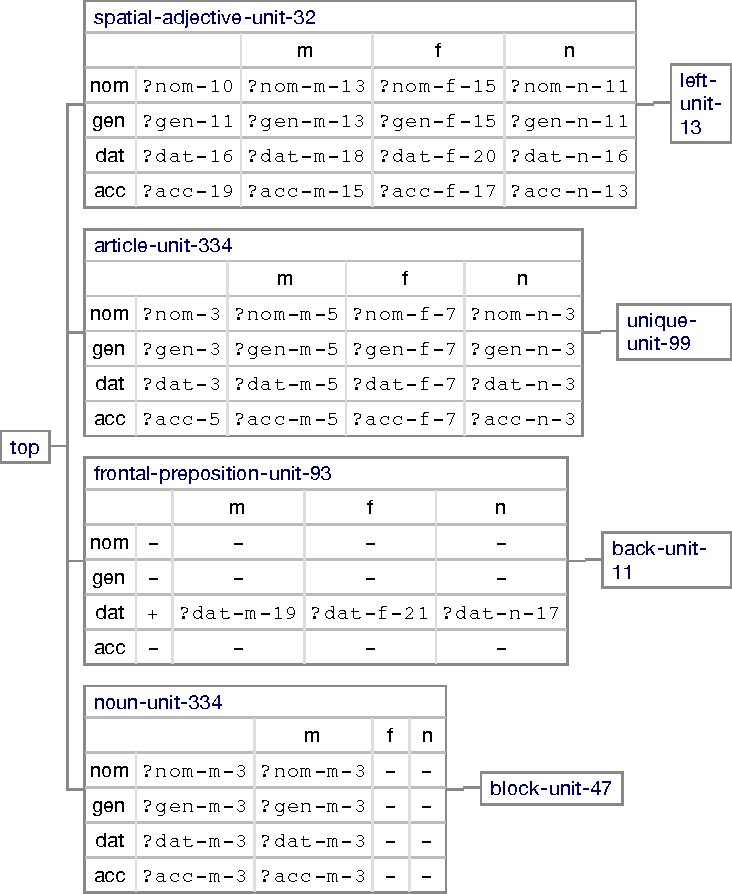
\includegraphics[scale=0.61]{figs/hinter-dem-linken-block-1}}
  \caption[Transient structure after the application of lexical and
    functional constructions]{Transient structure after the application of lexical and
    functional constructions for production of \textit{hinter dem linken
    Block} (`behind the left block'). For simplification, each unit
    is only shown with its distinctive feature matrix\index{design pattern!feature matrix} for case/gender
    agreement, if present. Furthermore, the feature matrices of the
    lexical units are identical to those of their parent units and are
    thus also not shown.}
  \label{f:hinter-dem-linken-block-1}
\end{figure}

\figref{f:hinter-dem-linken-block-1} shows the state of the
transient structure\index{transient structure} after the application of lexical and functional
constructions. It can be seen how the different states of information
for articles, adjectives, prepositions and nouns are technically
represented. The feature matrices\index{design pattern!feature matrix} for the spatial adjective
({\footnotesize\texttt{spatial-adjective-unit-334}}) and for the article
({\footnotesize\texttt{article-unit-334}}) are completely filled with variables. On
the other hand, the feature matrix\index{design pattern!feature matrix} for the frontal preposition
({\footnotesize\texttt{frontal-preposition-unit-93}}) features a `-' everywhere but
in the column representing the dative case, namely, the case it
requires. On the other hand, the noun ({\footnotesize\texttt{noun-unit-334}}) is
categorized based on its gender, and the feature matrix\index{design pattern!feature matrix} consequently
has variables in the row for masculine and excludes all other fields.

\subsection{Percolation and agreement -- moving information around and unification}
Given the setup of initial information by lexical and functional
constructions, all subsequently applied constructions have to be able
to move information around and to further constrain the
information. Movement of information is done using percolation, and
unification of feature matrices for agreement automatically constrains
the values in the feature matrices further and further.

\begin{figure}[t]
  \centerline{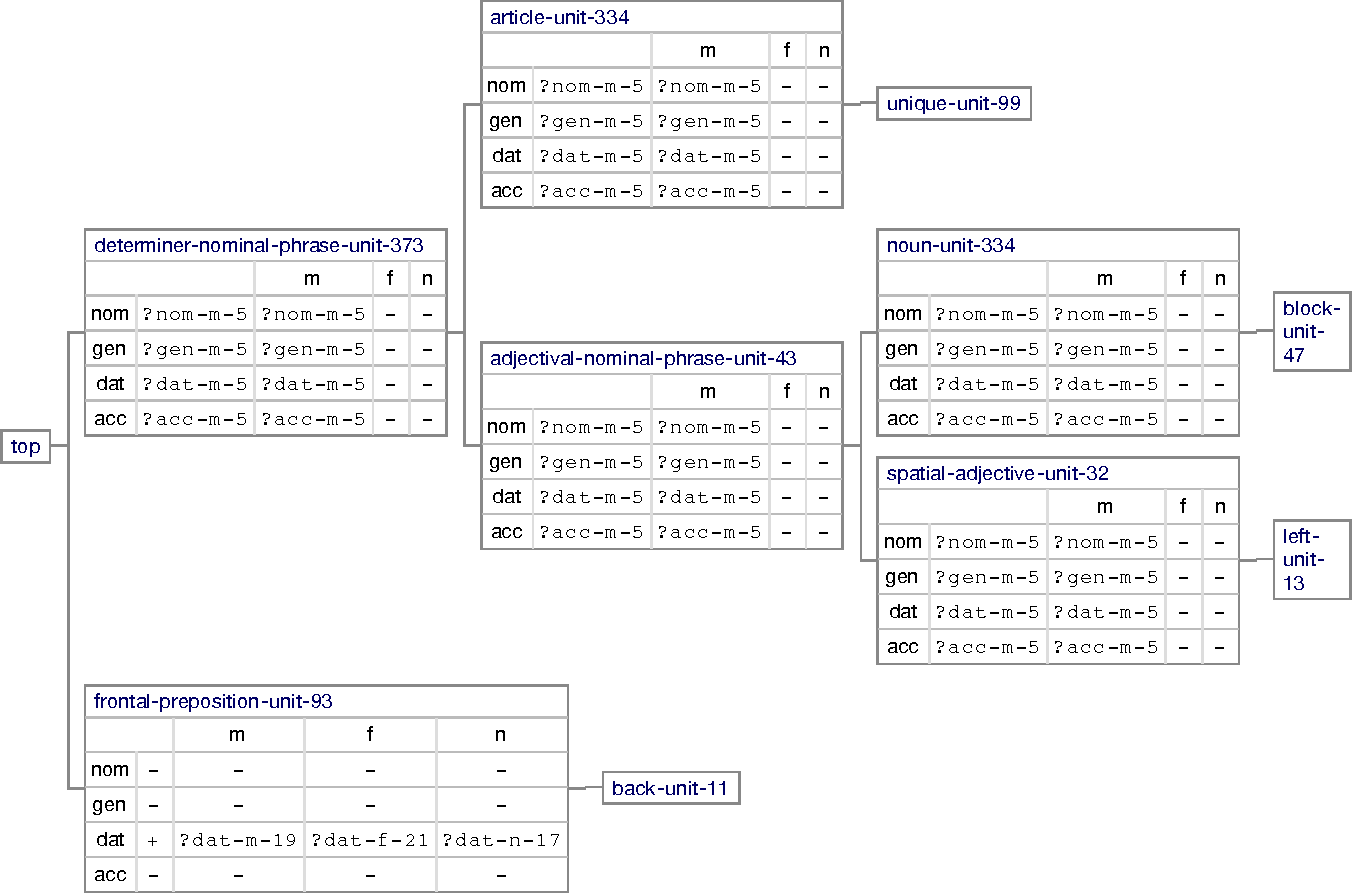
\includegraphics[scale=0.5]{figs/hinter-dem-linken-block-2}}
  \caption[Gender agreement represented in the transient structure]{
  Gender agreement 
  between the article, adjective and noun
  are enforced by the adjectival-nominal and
  determiner-nominal-phrase constructions applied to the transient
  structure in Figure \ref{f:hinter-dem-linken-block-1}. }
  \label{f:hinter-dem-linken-block-2}
\end{figure}

Both percolation and unification are used together, for instance, by
the {\footnotesize\tt adjectival-nominal} construction. (See Figure
\ref{f:hinter-dem-linken-block-2}.) In our example, this construction
handles the adjective ({\footnotesize\texttt{spatial-adjective-unit-334}}) and
the noun ({\footnotesize\texttt{noun-unit-334}}) as constituents. Apart from introducing
German word order, this construction unifies the feature matrix\index{design pattern!feature matrix} of the
adjective and the noun, which automatically constrains the gender
possibilities for the adjective, in this case, to masculine. In fact,
through unification the two feature matrices are the same after the
application of the {\footnotesize\tt adjectival-nominal}
constructions. Moreover, the newly created parent unit
({\footnotesize\texttt{adjectival-nominal-phrase-43}}) percolates this matrix
up. This process is subsequently repeated, this time by the
{\footnotesize\tt determiner-nominal} construction, which has the same effect
but this time with its constituents being the article and the
adjectival-nominal phrase, which also constrains the article to be
masculine. Percolation and unification have essentially
established the agreement between the article, the adjective and the
noun, while at the same time spreading the information about gender.


\begin{figure}[t]
  \centerline{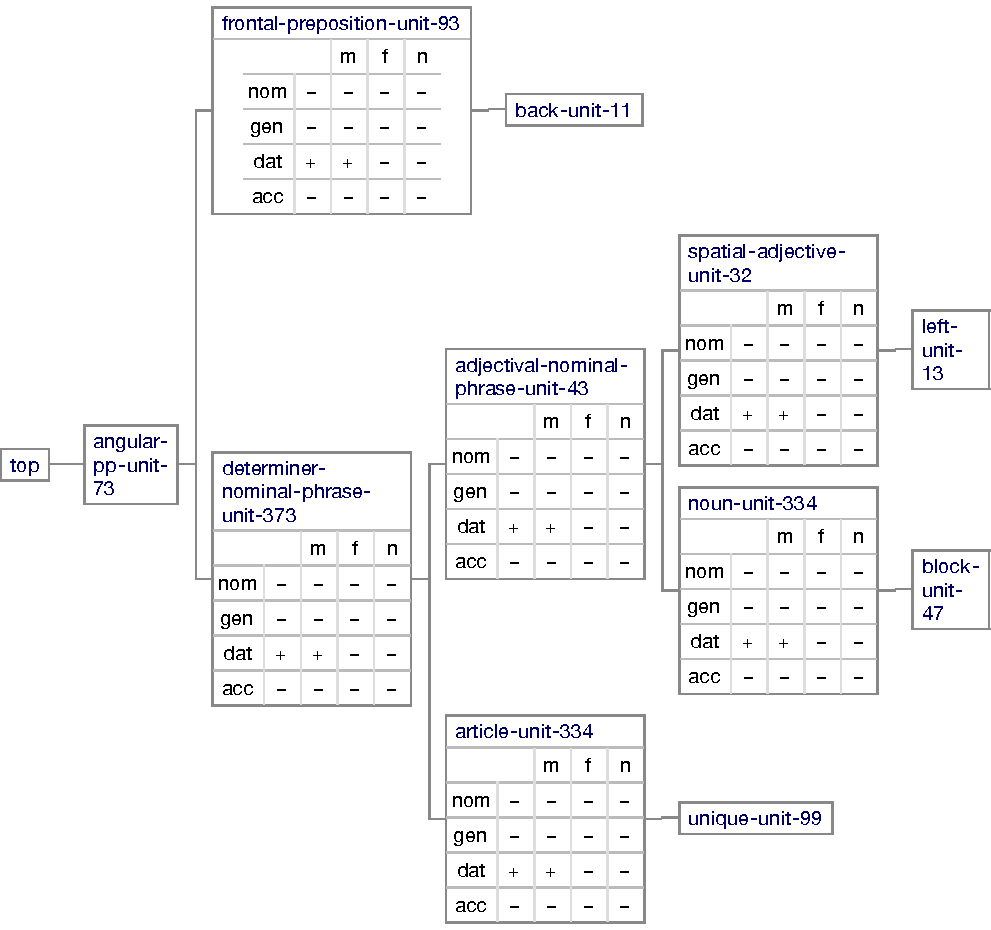
\includegraphics[scale=0.61]{figs/hinter-dem-linken-block-3}}
  \caption[Case agreement represented in the transient structure]{
  Case agreement after applying the angular-pp-phrase
    construction to the transient structure from Figure
    \ref{f:hinter-dem-linken-block-2} while producing ``hinter dem
    linken block''.}
  \label{f:hinter-dem-linken-block-3}
\end{figure}


After the application of these two constructions, the decision on case
is still missing. Case is provided by the angular preposition, and
agreement between the preposition and the determined-nominal-phrase is
established by the {\footnotesize\tt angular-pp-phrase}. (See Figure
\ref{f:hinter-dem-linken-block-3}). The {\footnotesize\tt angular-pp-phrase}
technically behaves very similarly to the the {\footnotesize\tt
  determiner-nominal} and the {\footnotesize\tt adjectival-nominal}
constructions: it unifies the feature matrices\index{design pattern!feature matrix} of its two constituents
({\footnotesize\texttt{frontal-preposition-unit-93}} and
{\footnotesize\texttt{determiner-nominal-phrase-unit-373}}).  However, the effect is
quite different in that now the feature matrix of the article, the
adjective and the noun is further constrained in terms of
case. Consequently, case and gender of this particular phrase are
ultimately decided.


\begin{figure}[t]
  \centerline{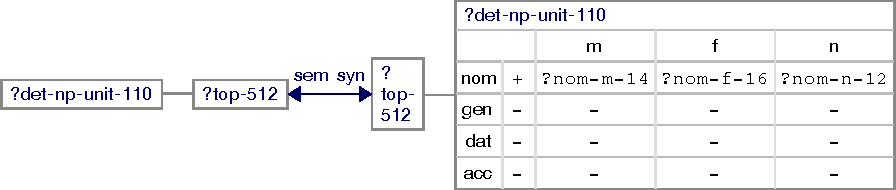
\includegraphics[scale=0.65]{figs/referring-expression-fvm}}
  \caption[Handling case in single determined-noun-phrases]{
  The referring-expression construction sets the case of a
    single determined-noun-phrase unit to nominative.}
  \label{f:referring-expression-fvm}
\end{figure}

For some phrases case is not established by prepositions but
rather by the general grammatical structure. A prime example is when 
the utterance itself only consists of a noun phrase, which then needs to be marked by 
the nominative case. For example when meanings for utterances such as \textit{der
linke Block} (`the block to the left') are expressed, then there
is no preposition that determines the case of the whole
phrase by agreement. Rather, the {\footnotesize\texttt{referring-expression}}
construction (see Figure \ref{f:referring-expression-fvm})
introduces the nominative case by unifying the feature matrix\index{design pattern!feature matrix} of the
determined-noun-phrase unit with a matrix constraining the case to
nominative.


\subsection{Postponing decisions}
After the application of the {\footnotesize\tt angular-pp-phrase}
construction, all necessary information has been accumulated. Case and
gender are decided, and, hence, all syntactic features for the
particular word class in question are available to allow subsequent
constructions to be able to decide the word form to be used. Morphological
constructions are used here to represent this relationship between syntactic
features and word forms. For example, for determiners, there
are six different articles in German that unevenly cover the 12
possible case-gender combinations, as shown in the chart below:

\begin{center}
  \begin{tabular}{cccc}
  	\lsptoprule
    & m & f & n \\ \midrule
    nom  & \emph{der} & \emph{die} & \emph{das} \\
    gen  & \emph{des} & \emph{der} & \emph{des} \\
    dat & \bf{\emph{dem}} & \emph{der} & \bf{\emph{dem}} \\
    acc & \emph{den} & \emph{die} & \emph{das} \\ 
	\lspbottomrule
  \end{tabular}
\end{center}
~\\

\begin{figure}[t]
  \centerline{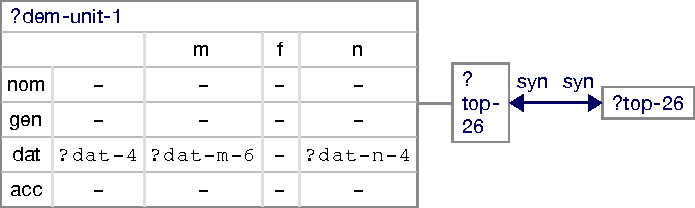
\includegraphics[scale=0.65]{figs/dem-morph-fvm}}
  \caption[Distinctive feature matrix\index{design pattern!feature matrix} of a morphological construction]{
  Distinctive feature matrix of the morphological construction
    that maps the string \textit{dem} to masculine or neuter and dative
    articles. Note that since this is a morphological construction, both
    poles of the construction apply to the syntactic pole of a transient
    structure.}
  \label{f:dem-morph}
\end{figure}

For each of these forms, a separate morphological construction exists
which decides on the form used to express the article
based on the lexical class and the case-gender feature matrix. An example of such a
morphological construction is shown in Figure \ref{f:dem-morph}. Since
this construction has a variable in the dative masculine field, it
matches with unit {\footnotesize\texttt{unique-unit-99}} in Figure
\ref{f:hinter-dem-linken-block-3}. Similarly, other morphological
entries add the strings \textit{linken} to the {\footnotesize\texttt{block-unit-47}},
\textit{Block} to the {\footnotesize\texttt{block-unit-47}} and \textit{hinter} to
{\footnotesize\texttt{back-unit-11}}.

%%%%%%%%%%%%%%%%%%%%%%%%%%%%%%%%%%%%
\begin{figure}
\begin{centering}
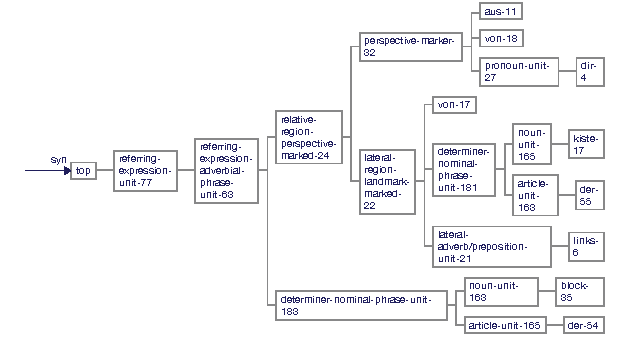
\includegraphics[width=\columnwidth]{figs/parse-result-transient-syn}
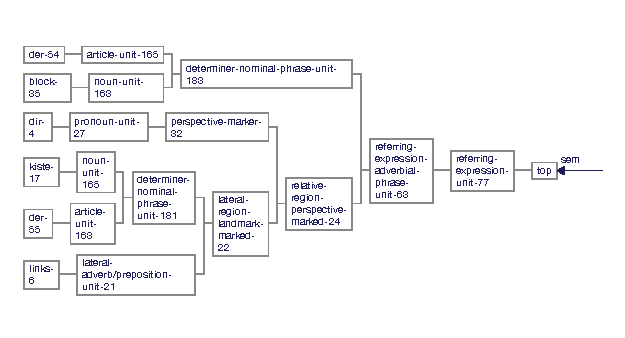
\includegraphics[width=\columnwidth]{figs/parse-result-transient-sem}
\caption[Final transient structure]{Parts of a final transient structure\index{transient structure}. The top shows the syntactic pole. The bottom
shows the semantic pole.}
\end{centering}
\label{f:parse-result-transient}
\end{figure}
\section{Summary}
Problems of intertwined information processing across multiple constructions 
and across different parts of transient structures often appear when dealing 
with complex, real world language. This chapter detailed how to tackle such 
problems using 1) adequate information representation techniques, such 
as logic variables, feature matrices\index{design pattern!feature matrix} and disjunctive potentials,
2) percolation for distributing information in the transient structure, and, 
3) special constructions which are needed to help postpone decisions until 
the state of information is ready. The techniques have proven to be 
sufficient for handling problems of syntactic indeterminacy, e.g., 
morphology and lexical class choice in German locative phrases. 
The discussed design patterns allow grammar 
designers to spread information processing across many constructions, 
leading to concise grammars, while facilitating efficient processing. 

The grammar is powerful enough to deal with German locative
phrases that include spatial relations, landmarks and even perspective.
Figure \ref{f:parse-result-transient} shows the final transient structure when an agent
parses the phrase \textit{der Block links von der Kiste von dir aus} (`the block
to the left of the box from your perspective').

%\bibliographystyle{diss}
%\bibliography{papers,space} 
%\end{document}